\documentclass[final]{beamer}

\usepackage[size=custom,width=120,height=90,scale=1.2]{beamerposter}
\usepackage{booktabs}
\usepackage[labelformat=empty]{caption}

\usetheme{default} % or try 'ConfPoster'

\title{Jazz Graph: \newline A Graph Neural Network for Jazz Music Recommendation}
\author{Stephen Lenhart \\ \texttt{lenhart.lenhart@gmail.com}}
\date{1 May 2026}
\institute{University of Arizona \newline College of Information Science}

%\setbeamerfont{title}{size=\Huge}
\setbeamerfont{title}{size=\fontsize{100}{110}\selectfont}

\begin{document}
	\begin{frame}[t]
		\vspace{-5em}
		\titlepage
		\vspace{-15em}
		\begin{columns}[t]
			
			% LEFT COLUMN
			\begin{column}{0.32\textwidth}
				\begin{block}{\Large Problem Statement}  % Name?
				Create musical recommendation by encoding collaboration as similarity signal.
				\begin{figure}
					
\includegraphics[width=\linewidth]{../poster_graph.png}
					\caption{A sub-graph illustrating connections among jazz performances. This is the one-hop neighborhood of the depicted performances. }
				\end{figure}
				\end{block}
				\begin{block}{Data}  
					\vspace{1em}
					\small
					\begin{center}
						
						\begin{tabular}{ll r r }
							
							\toprule
							Node/Edge Type & Count  & Mean degree  & Mean degree \\
							&           & source     & destination \\
							\midrule
							Artist                            &  24,470 & & \\
							Performance                       &  130,695 & \\
							Song                              &  31,828 & &  \\
							Artist \emph{performs} performance & 516,713 & 21.11 & 3.95 \\
							Performance \emph{performing} song & 86,588 & .66 &  2.72 \\
							Artist \emph{composed} song &        36,252 & 1.48 & 1.13 \\
							\bottomrule
						\end{tabular}
					\end{center}
					
					
				\end{block}
				\begin{block}{Graph Neural Network}
					JazzGraph GNN is a three-layer network for a heterogeneous graph; it combines GraphSAGE for featureless edges and GATv2Conv for artist-performance edges, which have an instrument feature.
				\end{block}
				\begin{block}{Training Task}
					Construct batches of positives pairs, where $x_i$, $x_j$ are positive if they are songs on the same album.
					Our loss function is computed as normalized temperature scaled cross-entropy loss:
					$$
					\mathcal{L}_{i, j} = -\log\frac{
						\exp(\text{sim}(z_i, z_j)/\tau)
					}{
						\sum_{k=1}^{2n} {\small [k\neq i]}\exp(\text{sim}(z_i, z_j) / \tau)
					}
					$$
					Where $\text{sim}$ is cosine similarity and $[k\neq i]$ is an indicator function equal to $1$ unless $k=i$, when it is $0$.
					
				\end{block}
				\begin{block}{Recommendation}
					Score each member of the performance corpus, $p_i$, with each seed performance (user-liked recording)  $$
					score(p_i) =  agg(\sum_{k=1}^{n}gnn(p_i)^\intercal gnn(p_k))
					$$
					where $gnn$ is the embedding learned from the graph of jazz performances, artists and songs and $agg$ is an aggregation or pooling function. Experiments were run with \emph{max}, \emph{sum} and \emph{softmax-weighting}.
					
				\end{block}
				
				
			\end{column}
			
			% MIDDLE COLUMN
			\begin{column}{0.32\textwidth}
				\vspace{10em}
				\begin{block}{\Large System Architecture}  % Methodology and Approach
					\begin{figure}
						\includegraphics[width=\linewidth]{../gnn_system}
						\caption{A data extraction pipeline(left), self-supervised learning with GNN (middle) and recommendation system (right.)}
					\end{figure}
				\end{block}
				\begin{block}{Repository}  
					\begin{figure}
						
\includegraphics[width=0.1\linewidth]{../repo_qr_code.png}
						\caption{https://www.github.com/philosofool/jazz-graph}
					\end{figure}
				\end{block}	
				\begin{block}{\Large Results}
				\begin{itemize}
					\item Novel Recall: Relevance of model recommendations.
					\item Novelty: Exploratory model behavior.
					\item B-Side: Expected recommendations for narrow seeds.
				\end{itemize}
				\vspace{1em}
				\small
				\begin{tabular}{ll l r r r r}
					\toprule
					Task & Features & Pooling & Novel Recall & Familiar Recall & Novelty & B-side Mean \\
					\midrule
					Combined Loss & Instrument, Style & sum     & 0.276 & 0.328 & 0.806 & 0.822 \\
					Combined Loss & Instrument, Style & max     & 0.297 & 1     & 0.840 & \textbf{0.839} \\
					Combined Loss & Instrument, Style & softmax & 0.276 & 0.318 & 0.807 & 0.822 \\
					
					Edge Ablation & Instrument, Style & sum     & 0.314 & 0.365 & 0.910 & 0     \\
					Edge Ablation & Instrument, Style & max     & 0.239 & 1     & \textbf{0.917} & 0 \\
					Edge Ablation & Instrument, Style & softmax & 0.323 & 0.393 & 0.910 & 0 \\
					
					Match Album & None & sum     & 0.278 & 0.378 & 0.850 & 0.434 \\
					Match Album & None & max     & 0.173 & 1     & 0.835 & 0.345 \\
					Match Album & None & softmax & 0.314 & 0.395 & 0.840 & 0.411 \\
					
					Match Album & Instrument, Style & sum     & 0.485 & 0.544 & 0.805 & 0.548 \\
					Match Album & Instrument, Style & max     & 0.295 & 1     & 0.829 & 0.523 \\
					Match Album & Instrument, Style & softmax & \textbf{0.518} & \textbf{0.608} & 0.804 & 0.548 \\
					
					Random Walk Baseline & --- & --- & 0.194 & 0.202 & 0.523 & 0.132 \\
					Artist Weighted Baseline & --- & --- & 0.420 & 0.405 & 0.011 & 0 \\
					\bottomrule
				\end{tabular}
				\end{block}
			\end{column}
			
			% RIGH COLUMN
			\begin{column}{0.32\textwidth}
				
%				
%				\begin{block}{Challenges and Limitations}  
%					Key takeaway here.
%				\end{block}
				\begin{block}{\Large Conclusions}
					\begin{itemize}
						\item Collaboration encodes useful similarity information.
						\item Recommendation strength depends on aggregation.
						\item Diversity in learned system is much better than baselines. 
						\item Many opportunities to improve the system.
					\end{itemize}  
					\begin{figure}
						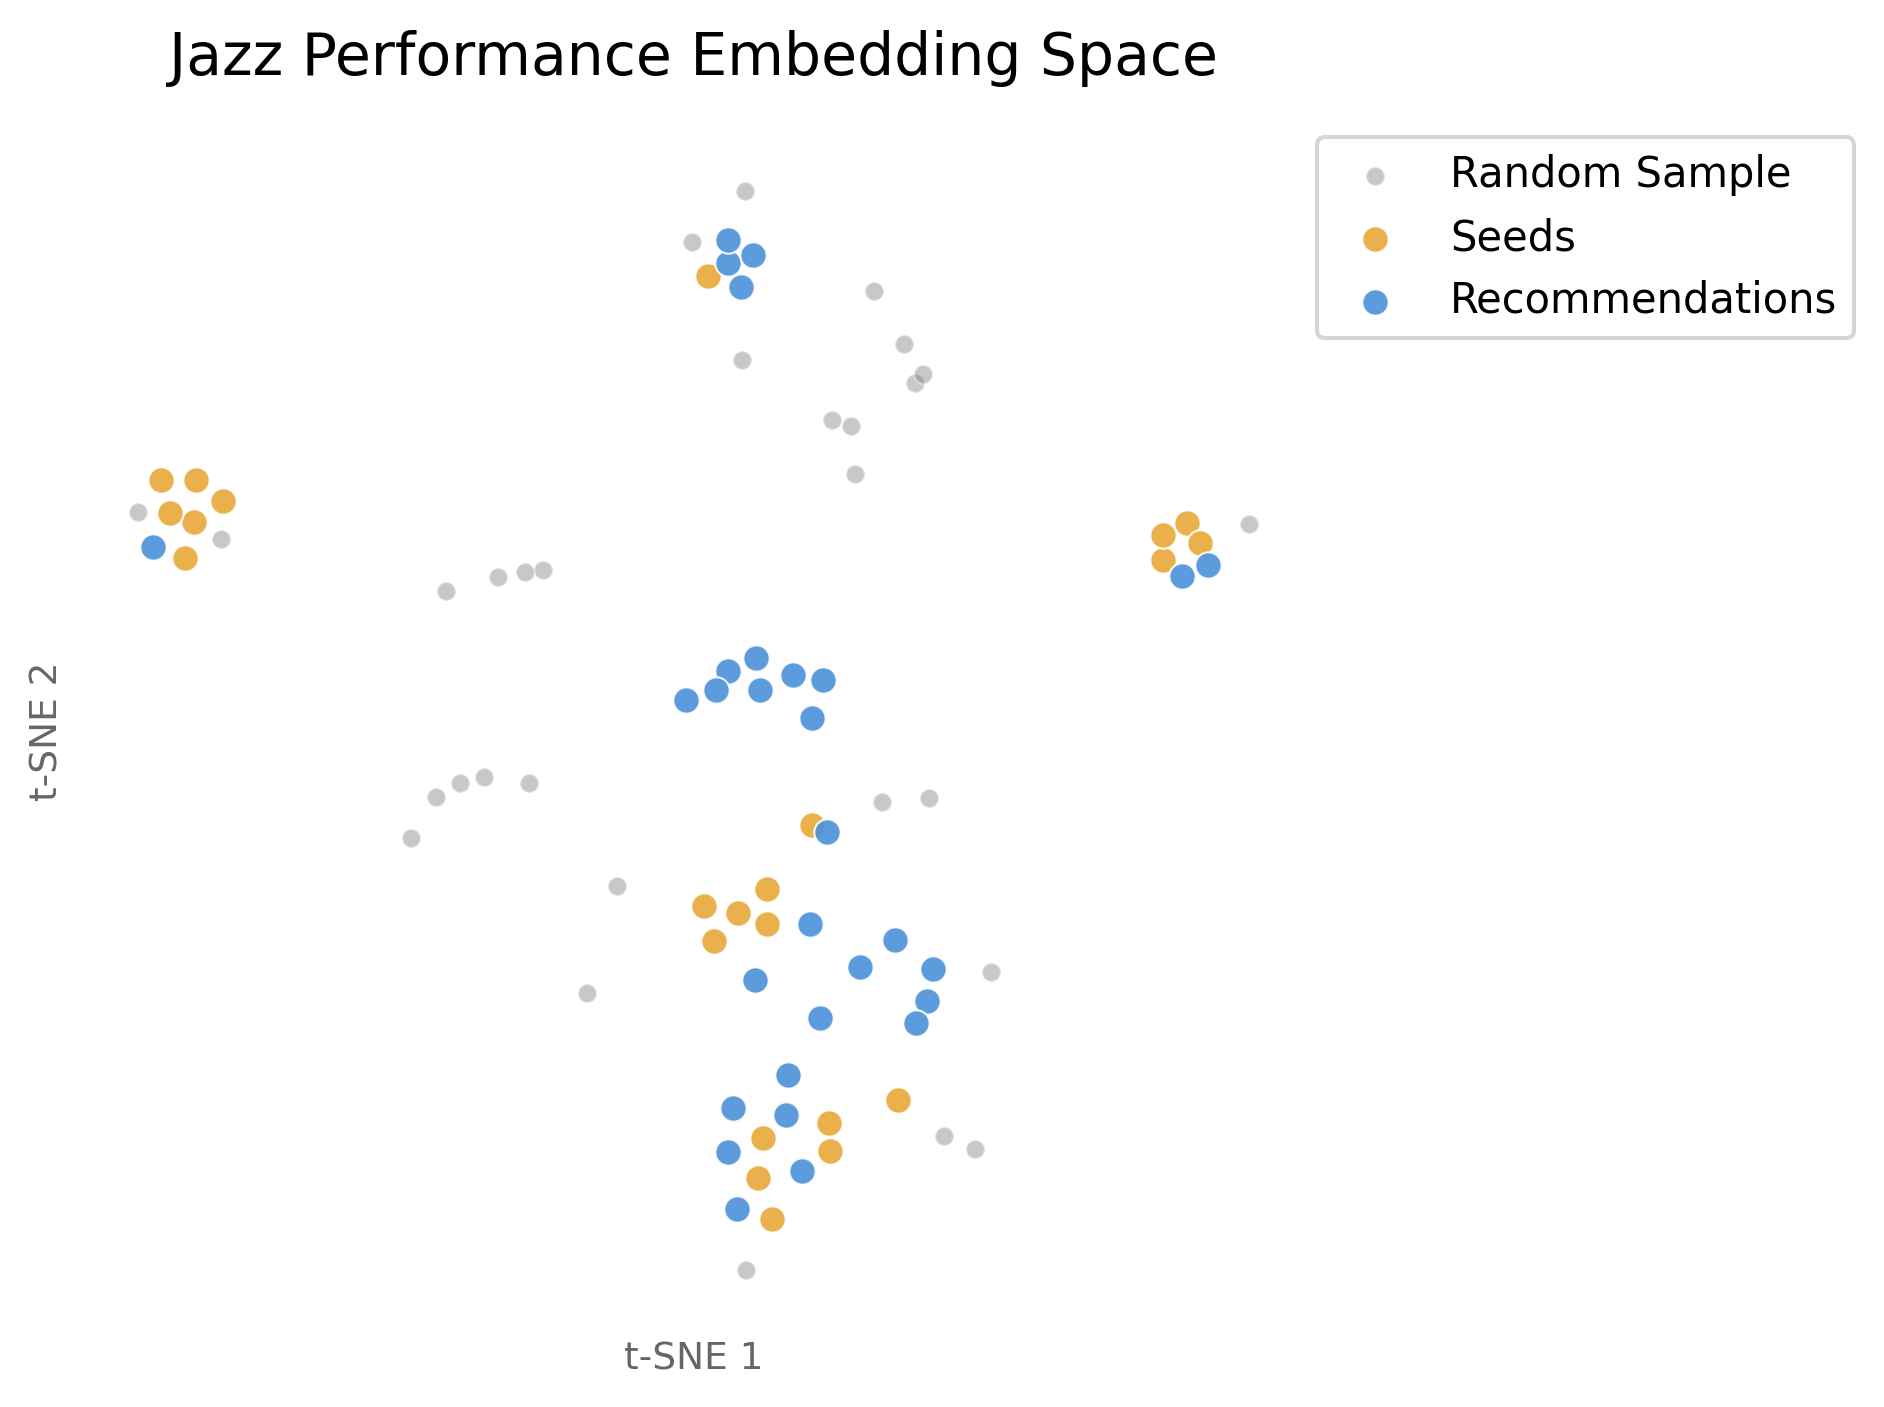
\includegraphics[width=\linewidth]{../jazz_performance_embeddings.png}
						\caption{t-SNE plot of the recommendations and seeds performances using 4 prominent jazz albums.}
					\end{figure}
				\end{block}	
%				
				\begin{block}{\Large Future Work}  
					\begin{itemize}
						\item Expand validations
						\item Provide additional features, such as session dates, mood, tempo
						\item Encode recordings as features
						\item Learn with Metapath2Vec or another algorithm
						\item Deploy system for public use
					\end{itemize}
				\end{block}
				
				\begin{block}{\Large Discovery}
						Listen to recommendations based on Joe Henderson's "Isotope":
						\begin{columns}
							\begin{column}{0.5\linewidth}
								\begin{figure}
									
\includegraphics[width=0.1\linewidth]{../spotify_playlist}
									\caption{Spotify}
								\end{figure}
							\end{column}
							\begin{column}{0.5\linewidth}
								\begin{figure}
									
\includegraphics[width=0.1\linewidth]{../apple_music_playlist}
									\caption{Apple Music}
								\end{figure}
							\end{column}
						\end{columns} 
					\begin{figure}
						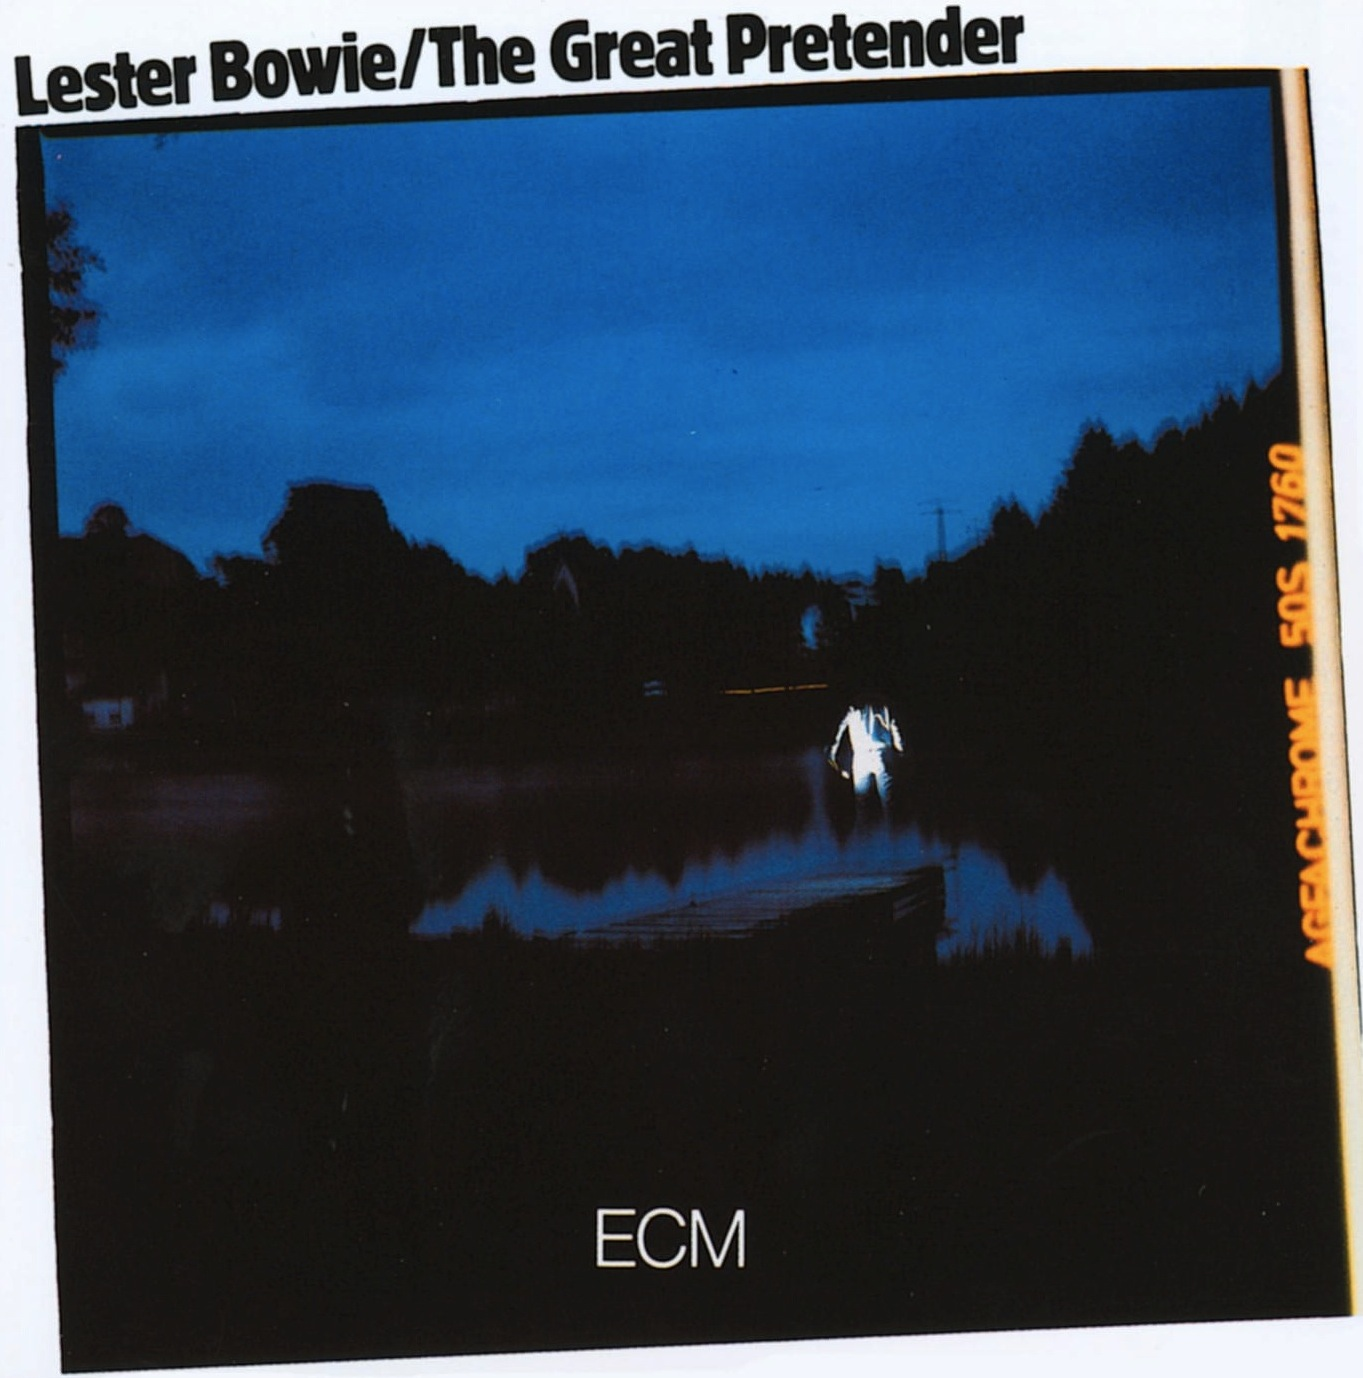
\includegraphics[width=0.3\linewidth]{../the-great-pretender3}
						\caption{Lester Bowie, "The Great Pretender" (1982) Great music I discovered with JazzGraph. }
					\end{figure}
				\end{block}
				
							
			\end{column}
			
		\end{columns}
	\end{frame}
	
\end{document}